\documentclass[a4paper,11pt]{article}
\usepackage{amsmath,amssymb}
\usepackage[a4paper,left=19mm,right=19mm,top=40mm,bottom=40mm]{geometry}
\usepackage{txfonts}
\usepackage{kotex}
\usepackage{graphicx}
\usepackage{algorithm}
\usepackage{algpseudocode}
\usepackage{fancyvrb}

\begin{document}
\title{자료구조 HW6}
\author{B935394 컴퓨터공학과 장준희}
\maketitle
\newpage
\section{Infix$\rightarrow$Postfix}
\begin{figure}[h]
\begin{center}
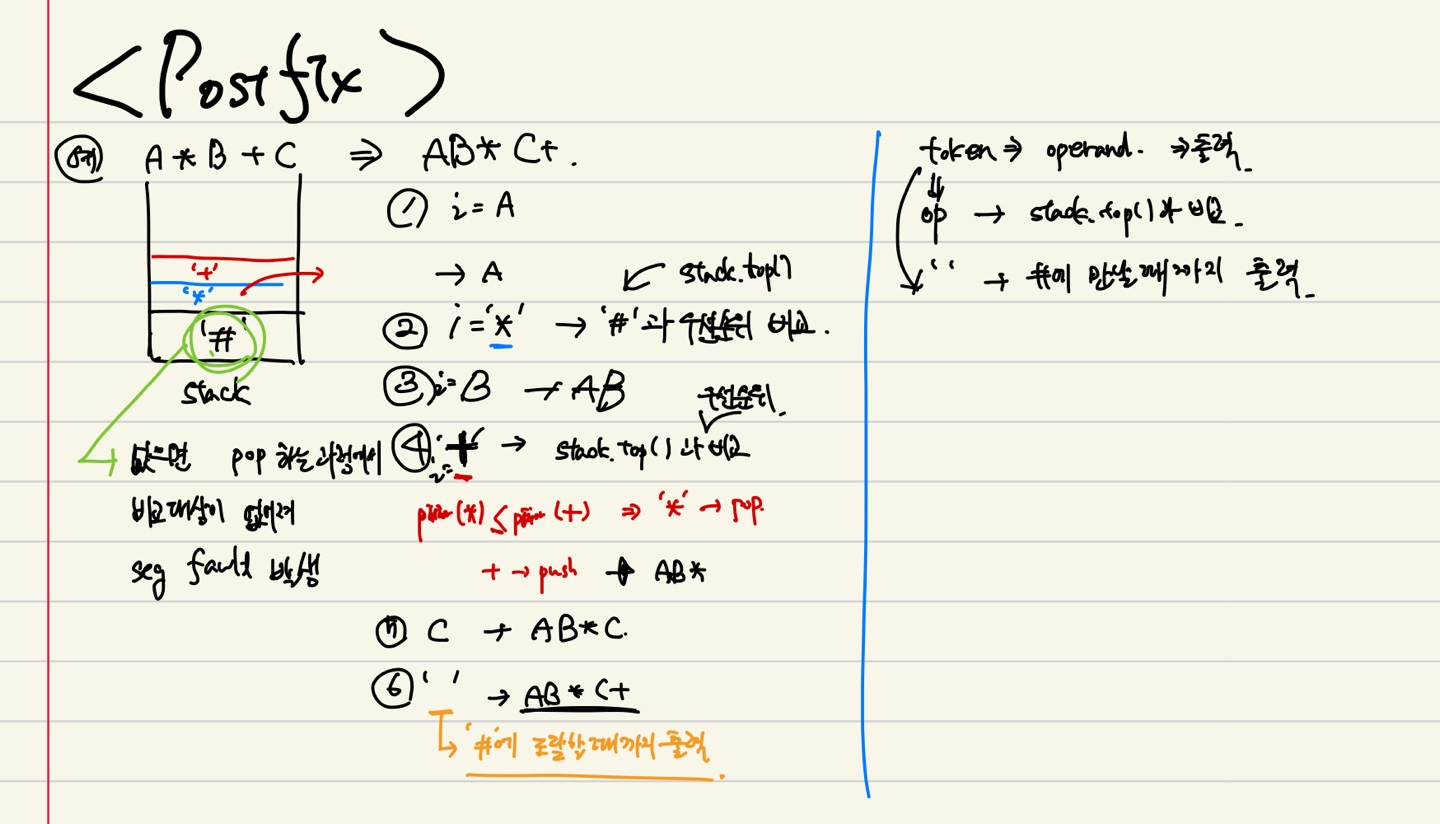
\includegraphics[width=\textwidth]{postfix}
\caption{Postfix}
\label{fig:fig1}
\end{center}
\end{figure}
\ref{fig:fig1}와 같이 간단한 예시를 들어서 설명을 해보면, 스택에 '\#'을 넣어둔 채로 문장을 앞에서부터 하나하나 읽는다. '\#'이 스택에 필요한 이유는 만약에 없다고 한다면, 우리가 나중에 operator의 우선순위를 비교해가며 pop()하고 push()를 할 떄, 스택이 텅 비어 비교할 때 접근하면 안되는 곳에 접근하기 때문이다. 우선순위로 비교를 하게될 것이기 때문에 '\#'에 할당되는 우선순위 값은 제일 커야한다.
\begin{enumerate}
\item 'A'입력 : 그대로 출력한다.
\item '*'입력 : '\#'과 우선순위를 비교, 더작으므로 그냥 push한다.
\item 'B'입력 : 그대로 출력한다.
\item '+'입력 : '*'와 우선순위 비교, 더 크므로 '*'을 출력, pop하고 '\#'과 우선순위 비교, 더 작으므로 push한다.
\item 'C'입력 : 그대로 출력한다.
\item ' '입력 : '\#'이 스택의 top이므로 멈춘다.
\end{enumerate}
\newpage
예시를 통해 알아본 것들을 정리하면,\\
\begin{enumerate}
\item 피연산자 입력 : 그대로 출력한다.
\item 연산자 입력 : stack의 top과 우선순위를 비교하고 그에 따라 동작을 정한다.
\item 공백 입력 : '\#'에 도달할 때까지 스택을 출력한다.\\
\end{enumerate}

코드로 구현하면 다음과 같다.
\\\begin{Verbatim}
------------------------------------------------------------------------
void Postfix(Expression e)  //program 3.19
{
    // infix expression e를 postfix form으로 바꾸어 출력
    // e에 토큰이 없으면 NextToken은 ‘#’ 토큰을 반환한다.
    // 스택의 밑에도 ‘#’를 넣고 시작한다.-->이게 없으면 아래의 문장들을
    // 실행할 때 공백인 상태에서 스택의 탑에 접근하는 경우가 생긴다.
    stack<Token> tokenStack;
    Token y;
    tokenStack.push('#');
    for(Token x = NextToken(e);x!='#';x=NextToken(e)){
        if(x.IsOperand()==true)     //x is operand
            cout<<x;
        else if(x==')'){         //x is parenthese, unstack until '('
            for(y=tokenStack.top();y!='(';y=tokenStack.top()){
                cout<<y;    tokenStack.pop();
            }
            tokenStack.pop();       //unstack '('
        }
        else{   //x is an operator
            for(y=tokenStack.top();isp(y)<=icp(x);y=tokenStack.top()){
                cout<<y;
                tokenStack.pop();
            }
            //tokenStack.push(y);       교재와는 달리 last y가 unstack되지 않는다.
            tokenStack.push(x);
        }           
    }
    while(tokenStack.top()!='#'){
        cout<<tokenStack.top();
        tokenStack.pop();
    }
    cout<<endl;     //pdf의 예상출력처럼 보기위해 개행
}
------------------------------------------------------------------------
\end{Verbatim}


\end{document}